\section{单纯逼近}
\sourcepage{93--94}
本节讨论，用单纯映射“逼近”任意连续映射的含义。

\entry{定义}{2.2.1}设 $h:|K|\to|L|$ 为连续映射。若对 $K$ 的每个顶点 $v$，存在 $L$ 的一个顶点 $w$，使
\[
h(\operatorname{St}v)\subset\operatorname{St}w,
\]
则称 $h$ 对 $K,L$ 满足\textbf{星形条件}（star condition）。

\entry{引理}{2.2.2}设 $h:|K|\to|L|$ 对 $K,L$ 满足星形条件。选择 $f:K^{(0)}\to L^{(0)}$，使每个顶点 $v$ 满足 $h(\operatorname{St}v)\subset\operatorname{St}f(v)$。则：
\begin{enumerate}[label=(\alph*)]
\item 给定 $\sigma\in K$，选取 $x\in\Int\sigma$，并选 $\tau$ 使 $h(x)\in\Int\tau$。则 $f$ 把 $\sigma$ 的每个顶点映到 $\tau$ 的某个顶点。
\item 函数 $f$ 能扩张为 $K\to L$ 的单纯映射，仍记为 $f$。
\item 若 $g:K\to L$ 是另一个满足 $h(\operatorname{St}v)\subset\operatorname{St}g(v)$ 的单纯映射，则 $f,g$ 邻接。
\end{enumerate}
\noindent\textbf{证明：}(a) 写 $\sigma=v_0\cdots v_p$。对每个 $i$，$x\in\operatorname{St}v_i$，故
\[
h(x)\in h(\operatorname{St}v_i)\subset\operatorname{St}f(v_i).
\]
\translatornote{原文此式第一个关系符误印为包含号；$h(x)$ 是点，应为属于号。}
因此 $h(x)$ 关于每个顶点 $f(v_i)$ 的重心坐标都为正，它们必为 $\tau$ 顶点集的子集。

(b) 因为 $f$ 把每个单形的顶点映为 $L$ 的某个单形的顶点，所以可扩张为单纯映射。

(c) 仍取上述 $\sigma,x,\tau$。对每个 $i$，有 $h(x)\in h(\operatorname{St}v_i)\subset\operatorname{St}g(v_i)$，故各 $g(v_i)$ 也是 $\tau$ 的顶点。因此所有 $f(v_i),g(v_i)$ 张成 $\tau$ 的一个面，$f,g$ 邻接。\hfill$\square$

\entry{定义}{2.2.3}设 $h:|K|\to|L|$ 连续。若单纯映射 $f:K\to L$ 对每个顶点 $v$ 满足 $h(\operatorname{St}v)\subset\operatorname{St}f(v)$，则称 $f$ 为 $h$ 的\textbf{单纯逼近}（simplicial approximation）。

\sourcepage{95--96}
在某种意义下，单纯逼近 $f$ 与 $h$ 很“接近”。更精确地说，对 $x\in|K|$，存在 $L$ 的某个单形同时包含 $h(x),f(x)$。

\entry{引理}{2.2.4}若 $f:K\to L$ 是 $h:|K|\to|L|$ 的单纯逼近，则对每个 $x\in|K|$，存在 $L$ 的单形 $\tau$，使 $h(x)\in\Int\tau$ 且 $f(x)\in\tau$。

\noindent\textbf{证明：}直接由引理 2.2.2(a) 得到。\hfill$\square$

\entry{定理}{2.2.5}设 $h:|K|\to|L|$、$k:|L|\to|M|$ 分别有单纯逼近 $f:K\to L$、$g:L\to M$，则 $g\circ f$ 是 $k\circ h$ 的单纯逼近。

\noindent\textbf{证明：}$g\circ f$ 当然为单纯映射。对 $K$ 的每个顶点 $v$，因为 $f$ 是逼近，有 $h(\operatorname{St}v)\subset\operatorname{St}f(v)$。又因为 $g$ 是逼近，
\[
k(h(\operatorname{St}v))\subset k(\operatorname{St}f(v))\subset\operatorname{St}g(f(v)).
\]\hfill$\square$

\entry{例}{2.2.6}设 $K,L$ 为图 2.2.1 的复形，底空间分别同胚于圆周和环带。按图示插入顶点，由 $K$ 得到复形 $K'$。设 $h$ 为图中连续映射，以 $A$ 表示 $h(a)$，其他顶点也类似。

$h$ 对 $K,L$ 不满足星形条件，但对 $K',L$ 满足，所以有单纯逼近 $f:K'\to L$。图中给出一个这样的逼近，以 $A'$ 表示 $f(a)$，其他顶点类似。
\begin{center}
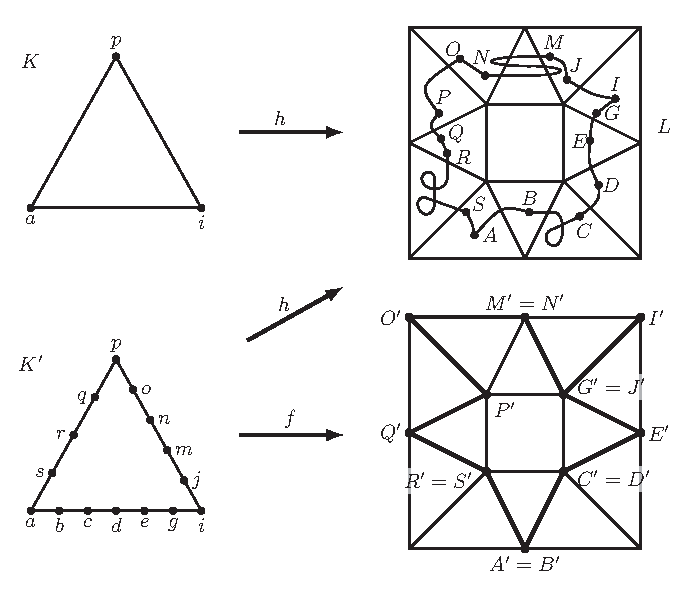
\includegraphics[width=119mm]{figures/2-2-1.pdf}\\图 2.2.1
\end{center}
若 $h$ 对 $K,L$ 满足星形条件，令 $h_*=f_*$，其中 $f$ 为任意单纯逼近，就得到良定义的同态 $h_*:H_p(K)\to H_p(L)$。容易看出它满足函子性质。

一般的连续映射 $h$ 不一定对 $K,L$ 满足星形条件，不能直接如此定义 $h_*$。怎么办？需要两个想法。

首先证明：给定 $h$，可将 $K$ “剖分”为底空间相同的新复形 $K'$，使 $h$ 对 $K',L$ 满足星形条件，正如例 2.2.6。此步骤是几何性的，将在第 2.3、2.4 节完成。

然后证明，恒等映射 $i:|K'|\to|K|$ 有一个诱导同调同构的单纯逼近 $g:K'\to K$。此步骤是代数性的，在第 2.5 节完成。最后定义
\[
h_*=f_*\circ g_*^{-1}:H_p(K)\to H_p(L).
\]
我们将在第 2.6 节看到，这个诱导同态也满足函子性质。

\subsection*{在相对同调中的应用}
上述单纯逼近结果直接推广到相对同调。

\entry{引理}{2.2.7}设 $h:|K|\to|L|$ 对 $K,L$ 满足星形条件，并将子复形的底空间 $|K_0|$ 映入 $|L_0|$。则：
\begin{enumerate}[label=(\alph*)]
\item 任意单纯逼近 $f:K\to L$ 也将 $|K_0|$ 映入 $|L_0|$，且其在 $K_0$ 上的限制是 $h|_{|K_0|}$ 的单纯逼近。
\item 任意两个单纯逼近 $f,g$ 作为偶的映射邻接。
\end{enumerate}
\sourcepage{97}
\noindent\textbf{证明：}给定 $\sigma\in K_0$，取 $x\in\Int\sigma$，令 $h(x)\in\Int\tau$。因为 $h$ 将 $|K_0|$ 映入 $|L_0|$，所以 $\tau\in L_0$。$f,g$ 都把 $\sigma$ 映到 $\tau$ 的面上，因此将 $K_0$ 映入 $L_0$，且作为偶的映射邻接。

再验证限制为单纯逼近。对 $K_0$ 的顶点 $v$，有 $\operatorname{St}(v,K_0)=\operatorname{St}(v,K)\cap|K_0|$，于是
\[
\begin{aligned}
h(\operatorname{St}(v,K_0))
&\subset h(\operatorname{St}(v,K))\cap h(|K_0|)\\
&\subset\operatorname{St}(f(v),L)\cap|L_0|\\
&=\operatorname{St}(f(v),L_0).
\end{aligned}
\]
得到所需结果。\hfill$\square$

下一个定义用于习题 2，并将在第 2.7 节再次出现。

\entry{定义}{2.2.8}映射 $f,h:X\to Y$ 之间的\textbf{同伦}（homotopy）是连续映射 $F:X\times I\to Y$，其中 $I=[0,1]$，使对每个 $x$ 有 $F(x,0)=f(x)$、$F(x,1)=h(x)$。下面 $(*)$ 定义的特定同伦称为\textbf{直线同伦}（straight-line homotopy）。

\subsection*{习题}
\begin{enumerate}
\item 考虑例 2.2.6 中的 $h:|K|\to|L|$，确定它有多少个不同的单纯逼近 $f:K'\to L$。设 $f,g$ 为两个逼近，选取生成 $H_1(K')$ 的闭链 $z$，找出 $L$ 的链 $d$，使 $\partial d=f_\#(z)-g_\#(z)$。\translatornote{原文选取闭链时误记为 $g$，与后面的公式不一致；这里统一为 $z$。}
\item \begin{enumerate}[label=(\alph*)]
\item 对映射 $f,h:X\to\R^N$，证明公式
\[
F(x,t)=(1-t)f(x)+th(x)\tag{$*$}
\]
定义两者之间的同伦，即直线同伦。
\item 设 $K,L$ 为 $\R^N$ 中的有限复形，$f:K\to L$ 为 $h:|K|\to|L|$ 的单纯逼近，证明 $(*)$ 定义两者之间的同伦。
\item[\textasteriskcentered\,(c)] 讨论 $K,L$ 不有限时的 (b)。
\end{enumerate}
\item 设 $f,h:\R\to\R^2$ 分别为 $f(x)=(x,x^3)$、$h(x)=(x,e^x)$，证明两者同伦。
\end{enumerate}
